\documentclass[../main.tex]{subfiles}
\graphicspath{{../image/}{../figure/}}
\begin{document}

\chapter{拉格朗日乘子}\label{appendix:c-拉格朗日乘子}

拉格朗日乘子也称拉格朗日乘数或未定乘子，用于在一个或多个约束条件下，寻找多变量函数的驻点。考虑在与 $x_1,x_2$ 有关的约束条件下找到函数 $f(x_1,x_2)$ 最大值的问题。该约束条件可以写成如下形式：
\begin{align}
g(x_1,x_2)=0
\label{align:appC-constraint}
\end{align}

一种方法是求解约束方程 [式~\eqref{align:appC-constraint}]，从而将 $x_2$ 表示为 $x_1$ 的函数，形式为 $x_2=h(x_1)$。然后将其代入 $f(x_1,x_2)$，得到形式为 $f(x_1,h(x_1))$ 的仅关于 $x_1$ 的函数。接下来，可以通过常用的微分方法找到关于 $x_1$ 的最大值，得到驻点值 $x_1^{*}$，相应的 $x_2^{*}$ 值由 $x_2^{*}=h(x_1^{*})$ 给出。

这种方法存在的一个问题是，找到约束方程的一个解析解可能会很困难（该方程使得 $x_2$ 可以表示为 $x_1$ 的显式函数）。此外，这种方法区别对待 $x_1$ 和 $x_2$，因而会破坏这些变量之间的自然对称性。

一种更优雅且通常更简单的方法是引入一个称为\textbf{拉格朗日乘子}的参数 $\lambda$。我们将从几何角度来说明这一技术。考虑一个具有 $x_1,\cdots,x_D$ 分量的 $D$ 维向量 $x$。约束方程 $g(x)=0$ 表示 $x$ 空间中的一个 $(D-1)$ 维曲面。如果 $x$ 是 $D$ 维的，则约束条件 $g(x)=0$ 对应一个维度为 $D-1$ 的子空间。我们想在约束条件 $g(x)=0$ 下最大化函数 $f(x)$。

\begin{figure}[htbp]
\centering
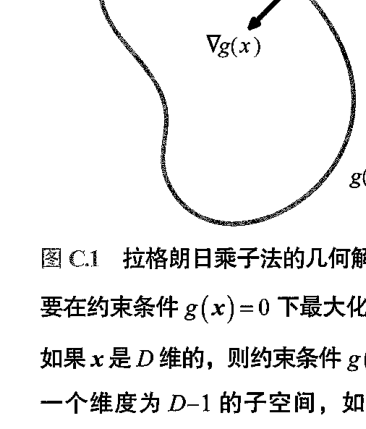
\includegraphics[width=0.6\textwidth]{appC-fig556-lagrange.png}
\caption{拉格朗日乘子法的几何解释。我们想要在约束条件 $g(x)=0$ 下最大化函数 $f(x)$。约束曲面上任何一点，约束函数的梯度 $\nabla g(x)$ 都与曲面正交；在约束曲面上使 $f(x)$ 最大的点 $x^{*}$ 处，$\nabla f(x^{*})$ 也与约束曲面垂直，因此 $\nabla f$ 与 $\nabla g$ 平行。}
\label{fig:appC-lagrange}
\end{figure}

首先注意，在该约束曲面上的任何一点，约束函数的梯度 $\nabla g(x)$ 都与曲面正交。为了说明这一点，考虑一个位于该约束曲面上的点 $x$ 以及另一个位于该约束曲面上的附近点 $x+\epsilon$。如果我们在点 $x$ 附近进行泰勒展开，则有
\begin{align}
g(x+\epsilon)\approx g(x)+\epsilon^{\mathsf{T}}\nabla g(x)
\end{align}
因为点 $x$ 和点 $x+\epsilon$ 都位于约束曲面上，所以我们有 $g(x)=g(x+\epsilon)$，从而有 $\epsilon^{\mathsf{T}}\nabla g(x)\approx 0$。当 $\epsilon\to 0$ 时，我们有 $\epsilon^{\mathsf{T}}\nabla g(x)=0$，并且因为 $\epsilon$ 与约束曲面 $g(x)=0$ 平行，所以我们看到 $\nabla g$ 与约束曲面是垂直的。

接下来我们寻找约束曲面上使得 $f(x)$ 最大化的点 $x^{*}$。这样的点满足 $\nabla f(x^{*})$ 也与约束曲面垂直的性质，否则我们可以通过沿约束曲面移动一小段距离来增大 $f(x)$ 的值。因此，$\nabla f$ 和 $\nabla g$ 是平行（或反平行）的，并且必定存在一个参数 $\lambda$，使得
\begin{align}
\nabla f+\lambda\nabla g=0
\label{align:appC-stationary}
\end{align}
其中 $\lambda\neq 0$ 称为拉格朗日乘子。注意，$\lambda$ 可正可负。

至此，我们很容易引出下式定义的\textbf{拉格朗日函数}（Lagrangian）：
\begin{align}
L(x,\lambda)=f(x)+\lambda g(x)
\label{align:appC-lagrangian}
\end{align}
为了找到在约束条件 $g(x)=0$ 下函数 $f(x)$ 的最大值，首先定义式~\eqref{align:appC-lagrangian} 所示的拉格朗日函数，然后寻找 $L(x,\lambda)$ 关于 $x$ 和 $\lambda$ 的驻点。对于一个 $D$ 维向量 $x$，这会给出 $D+1$ 个方程，用于确定驻点 $x^{*}$ 以及 $\lambda^{*}$ 的值。可通过设置 $\nabla L=0$ 得到带约束的驻点条件 [式~\eqref{align:appC-stationary}]。此外，通过 $\partial L/\partial\lambda=0$ 可推出约束条件 $g(x)=0$。如果只对 $x$ 感兴趣，则可以从驻点方程中消去 $\lambda$，而不需要计算 $\lambda$ 的值（``未定乘子''由此得名）。

\begin{figure}[htbp]
\centering
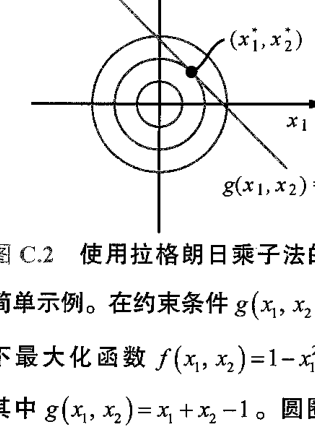
\includegraphics[width=0.6\textwidth]{appC-fig557-example.png}
\caption{使用拉格朗日乘子法的一个简单示例。在约束条件 $g(x_1,x_2)=0$ 下最大化函数 $f(x_1,x_2)=1-x_1^2-x_2^2$，其中 $g(x_1,x_2)=x_1+x_2-1$。椭圆表示函数 $f(x_1,x_2)$ 的等值线，对角线则代表约束曲面 $g(x_1,x_2)=0$。}
\label{fig:appC-example}
\end{figure}

举个简单的例子，假设我们希望找到函数 $f(x_1,x_2)=1-x_1^2-x_2^2$ 在约束条件 $g(x_1,x_2)=x_1+x_2-1=0$ 下的驻点。相应的拉格朗日函数由下式给出：
\begin{align}
L(x,\lambda)=1-x_1^2-x_2^2+\lambda(x_1+x_2-1)
\label{align:appC-example-lag}
\end{align}
这个拉格朗日函数关于 $x_1$、$x_2$ 和 $\lambda$ 的驻点条件给出了如下耦合方程：
\begin{align}
-2x_1+\lambda=0
\label{align:appC-ex1}
\end{align}
\begin{align}
-2x_2+\lambda=0
\label{align:appC-ex2}
\end{align}
\begin{align}
x_1+x_2-1=0
\label{align:appC-ex3}
\end{align}
解这些方程，可以得到驻点 $(x_1^{*},x_2^{*})=(1/2,1/2)$，相应的拉格朗日乘子为 $\lambda=1$。

到目前为止，我们已经讨论了在形如 $g(x)=0$ 的\textbf{等式约束}（equality constraint）下如何最大化函数的问题。接下来考虑在形如 $g(x)\ge 0$ 的\textbf{不等式约束}（inequality constraint）下如何最大化 $f(x)$ 的问题。

根据带约束的驻点是否位于 $g(x)>0$ 的区域内，这个问题有两种可能的解。如果驻点位于 $g(x)>0$ 的区域内，则约束是\textbf{非激活的}（inactive）；而如果驻点位于边界 $g(x)=0$ 上，则约束是\textbf{激活的}（active）。在前一种情况下，函数 $g(x)$ 不起作用，因此驻点条件是 $\nabla f(x)=0$，这对应于 $\lambda=0$ 的拉格朗日函数 [式~\eqref{align:appC-lagrangian}] 的驻点。在后一种情况下，驻点位于边界上，类似于前面讨论的等式约束，对应于 $\lambda\neq 0$ 的拉格朗日函数 [式~\eqref{align:appC-lagrangian}] 的驻点。可见拉格朗日乘子的符号是关键，因为只有当 $f(x)$ 的梯度远离 $g(x)>0$ 的区域时，函数 $f(x)$ 才会达到最大值。因此，当 $\lambda>0$ 时，我们有 $\nabla f(x^{*})=-\lambda\nabla g(x^{*})$。

\begin{figure}[htbp]
\centering
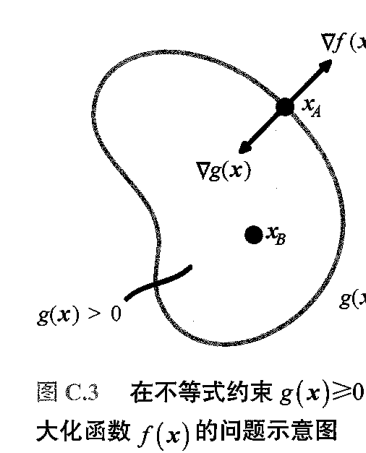
\includegraphics[width=0.6\textwidth]{appC-fig558-inequality.png}
\caption{在不等式约束 $g(x)\ge 0$ 下最大化 $f(x)$ 的问题示意图。当驻点位于 $g(x)>0$ 的区域内时约束非激活；当驻点位于 $g(x)=0$ 的边界上时约束激活。}
\label{fig:appC-inequality}
\end{figure}

对于这两种情况，乘积 $\lambda g(x)=0$。因此，在 $g(x)\ge 0$ 的不等式约束下最大化 $f(x)$ 的问题，可通过在以下条件下关于 $x$ 和 $\lambda$ 优化拉格朗日函数 [式~\eqref{align:appC-lagrangian}] 来求解：
\begin{align}
g(x)\ge 0
\label{align:appC-kkst1}
\end{align}
\begin{align}
\lambda\ge 0
\label{align:appC-kkst2}
\end{align}
\begin{align}
\lambda g(x)=0
\label{align:appC-kkst3}
\end{align}
我们称它们为\textbf{卡鲁什-库恩-塔克}（Karush-Kuhn-Tucker, KKT）条件（Karush, 1939; Kuhn and Tucker, 1951）。注意，如果我们希望在不等式约束 $g(x)\ge 0$ 下最小化（而非最大化）函数 $f(x)$，则需要关于 $x$ 最小化拉格朗日函数 $L(x,\lambda)=f(x)-\lambda g(x)$，这同样要求 $\lambda\ge 0$。

最后，拉格朗日乘子法可以很容易地扩展到具有多个等式约束和不等式约束的情况。假设我们希望在约束条件 $g_j(x)=0$（$j=1,\cdots,J$）和 $h_k(x)\ge 0$（$k=1,\cdots,K$）下最大化 $f(x)$，则可以引入拉格朗日乘子 $\{\lambda_j\}$ 和 $\{\mu_k\}$，并优化如下拉格朗日函数：
\begin{align}
L(x,\{\lambda_j\},\{\mu_k\})=f(x)+\sum_j \lambda_j g_j(x)+\sum_k \mu_k h_k(x)
\label{align:appC-general}
\end{align}
其中 $\mu_k\ge 0$ 且 $\mu_k h_k(x)=0$，$k=1,\cdots,K$。关于拉格朗日乘子法更详细的讨论，请参阅 Nocedal and Wright (1999)。

\end{document}